\documentclass{beamer}
\usetheme{metropolis}           % Use metropolis theme
\metroset{numbering=fraction}
\usepackage{tikz}
\usetikzlibrary{arrows,positioning,shapes.geometric}
\usepackage{float}
\usepackage{makecell}
\usepackage{fancyvrb}
\usepackage{listings}
\usepackage[export]{adjustbox}
\usepackage{caption}
\title{Lecture 2.1 \\ Introduction to Object-Oriented Programming (OOP)}
\date{\today}
\author{Michael Giannikouris}
\institute{Department of Electrical and Computer Engineering}
\setbeamertemplate{caption}{\raggedright\insertcaption\par}
\setbeamersize{text margin left=12pt,text margin right=12pt}
\newcommand{\putat}[3]{\begin{picture}(0,0)(0,0)\put(#1,#2){#3}\end{picture}} % just a shorthand

\newenvironment{deflist}
{ \begin{description}
    \setlength{\itemsep}{6pt}
    \setlength{\parskip}{0pt}
    \setlength{\parsep}{0pt}     }
{ \end{description}                  } 

\newenvironment{splitslide}
{
\centering
\begin{tabular}{@{}p{0.50\textwidth} | p{0.025\textwidth}@{} p{0.4\textwidth}@{}}
}
{
\end{tabular}
}


\begin{document}
\maketitle

\section{Characteristics of OOP}

%%%%%%%%%%%%%%%%%%%%%%%%%%%%%%%%%%%%%%%%%%%%%%%%%%%%%%%%%%%%%%%%%%%%%%%%%%%%%%%%%%%%
% Encapsulation (Definition)
%%%%%%%%%%%%%%%%%%%%%%%%%%%%%%%%%%%%%%%%%%%%%%%%%%%%%%%%%%%%%%%%%%%%%%%%%%%%%%%%%%%%
\begin{frame}{Characteristics of OOP}
	\begin{deflist}
		\item[Encapsulation]
		Data and methods that operate on the data are \textbf{bundled} together in a single container.	
		\item Some of the data and methods internal to the container may be hidden, depending on their \textbf{visibility}.
		\item[] Typically, OOP languages (including Java) call this container a \textbf{class}.
	\end{deflist}
\end{frame}
%%%%%%%%%%%%%%%%%%%%%%%%%%%%%%%%%%%%%%%%%%%%%%%%%%%%%%%%%%%%%%%%%%%%%%%%%%%%%%%%%%%%



%%%%%%%%%%%%%%%%%%%%%%%%%%%%%%%%%%%%%%%%%%%%%%%%%%%%%%%%%%%%%%%%%%%%%%%%%%%%%%%%%%%%
% Encapsulation (Bundling)
%%%%%%%%%%%%%%%%%%%%%%%%%%%%%%%%%%%%%%%%%%%%%%%%%%%%%%%%%%%%%%%%%%%%%%%%%%%%%%%%%%%%
\begin{frame}[fragile]{Encapsulation}

\centering
\begin{tabular}{@{}m{0.50\textwidth} | m{0.03\textwidth}@{} m{0.4\textwidth}@{}}

\begin{Verbatim}[fontsize=\tiny]
public class BankAccount {
  public double balance;
  
  // constructor
  public BankAccount(double opening_balance) {
    balance = opening_balance;
  }
  
  // deposit an amount
  public void deposit(double amount) {
    balance += amount;
  }
  
  // withdraw an amount
  public boolean withdraw(double amount) {
    if(balance < amount) {
      return false;
    }
    else {
      balance -= amount;
      return true;
    }
  }
}
\end{Verbatim}

&&

\raggedright
\begin{footnotesize}
Data (\textbf{balance}) 	\\
and methods (\textbf{deposit}, \textbf{withdraw})	\\
are \textbf{bundled} into a single container, the BankAccount \textbf{class}. \\
\end{footnotesize}

\end{tabular}

\end{frame}
%%%%%%%%%%%%%%%%%%%%%%%%%%%%%%%%%%%%%%%%%%%%%%%%%%%%%%%%%%%%%%%%%%%%%%%%%%%%%%



%%%%%%%%%%%%%%%%%%%%%%%%%%%%%%%%%%%%%%%%%%%%%%%%%%%%%%%%%%%%%%%%%%%%%%%%%%%%%%
% Encapsulation (Visibility)
%%%%%%%%%%%%%%%%%%%%%%%%%%%%%%%%%%%%%%%%%%%%%%%%%%%%%%%%%%%%%%%%%%%%%%%%%%%%%%
\begin{frame}[fragile]{Encapsulation}

\centering
\begin{tabular}{@{}m{0.50\textwidth} | m{0.03\textwidth}@{} m{0.4\textwidth}@{}}

\begin{Verbatim}[fontsize=\tiny]
public class BankAccount {
  public double balance;
  
  // constructor
  public BankAccount(double opening_balance) {
    balance = opening_balance;
  }
  
  // deposit an amount
  public void deposit(double amount) {
    balance += amount;
  }
  
  // withdraw an amount
  public boolean withdraw(double amount) {
    if(balance < amount) {
      return false;
    }
    else {
      balance -= amount;
      return true;
    }
  }
}
\end{Verbatim}

&&

\raggedright
\begin{footnotesize}
Notice that we've put \textbf{public} in front of all of our data and methods (and the class itself). \\
\vspace{0.5em}
Public is one of Java's \textbf{access modifier} keywords. \\
\vspace{0.5em}
These keywords control the \textbf{visibility} of class members (and classes themselves). 
\end{footnotesize}

\end{tabular}

\end{frame}
%%%%%%%%%%%%%%%%%%%%%%%%%%%%%%%%%%%%%%%%%%%%%%%%%%%%%%%%%%%%%%%%%%%%%%%%%%%%%%%%%%%%



%%%%%%%%%%%%%%%%%%%%%%%%%%%%%%%%%%%%%%%%%%%%%%%%%%%%%%%%%%%%%%%%%%%%%%%%%%%%%%%%%%%%
% Java Access Modifiers 
%%%%%%%%%%%%%%%%%%%%%%%%%%%%%%%%%%%%%%%%%%%%%%%%%%%%%%%%%%%%%%%%%%%%%%%%%%%%%%%%%%%%
\begin{frame}[fragile]{Java Access Modifiers}
\begin{center}
\begin{tabular}{ l | l | l | l | l }
\textbf{Modifier} & \textbf{Class} & \textbf{Package} & \textbf{Subclass} & \textbf{World} \\
\hline
public & Y & Y & Y & Y \\
\hline
protected & Y & Y & Y & N \\
\hline
\textit{no modifier} & Y & Y & N & N \\
\hline
private & Y & N & N & N \\
\end{tabular}
\end{center}
\end{frame}
%%%%%%%%%%%%%%%%%%%%%%%%%%%%%%%%%%%%%%%%%%%%%%%%%%%%%%%%%%%%%%%%%%%%%%%%%%%%%%%%%%%%



%%%%%%%%%%%%%%%%%%%%%%%%%%%%%%%%%%%%%%%%%%%%%%%%%%%%%%%%%%%%%%%%%%%%%%%%%%%%%%
% Encapsulation (Choosing Good Visibility)
%%%%%%%%%%%%%%%%%%%%%%%%%%%%%%%%%%%%%%%%%%%%%%%%%%%%%%%%%%%%%%%%%%%%%%%%%%%%%%
\begin{frame}[fragile]{Encapsulation}

\centering
\begin{tabular}{@{}m{0.50\textwidth} | m{0.03\textwidth}@{} m{0.4\textwidth}@{}}

\begin{Verbatim}[fontsize=\tiny]
public class BankAccount {
  private double balance;
  
  // constructor
  public BankAccount(double opening_balance) {
    balance = opening_balance;
  }
  
  // deposit an amount
  public void deposit(double amount) {
    balance += amount;
  }
  
  // withdraw an amount
  public boolean withdraw(double amount) {
    if(balance < amount) {
      return false;
    }
    else {
      balance -= amount;
      return true;
    }
  }
\end{Verbatim}

&&

\raggedright
\begin{footnotesize}
Visibility is very important when designing a class.\\
\vspace{0.5em}
For example, we probably don't want users to be able to directly change \textbf{balance}, so we'll make it \textbf{private}. \\
\vspace{0.5em}
In general, use the most restrictive access level possible. \\
\end{footnotesize}

\end{tabular}

\end{frame}
%%%%%%%%%%%%%%%%%%%%%%%%%%%%%%%%%%%%%%%%%%%%%%%%%%%%%%%%%%%%%%%%%%%%%%%%%%%%%%%%%%%%



%%%%%%%%%%%%%%%%%%%%%%%%%%%%%%%%%%%%%%%%%%%%%%%%%%%%%%%%%%%%%%%%%%%%%%%%%%%%%%%%%%%%
% Inheritence 
%%%%%%%%%%%%%%%%%%%%%%%%%%%%%%%%%%%%%%%%%%%%%%%%%%%%%%%%%%%%%%%%%%%%%%%%%%%%%%%%%%%%
\begin{frame}{Characteristics of OOP}
	\begin{deflist}
		\item[Inheritance]
		Classes can \textbf{extend} (build on) other classes.
		\item[] A "child" class inherits (some of) the data and methods of the "parent" class.	
		\item[] A "child" class can also add new data and methods.
		\item[] In Java, we usually use the terms \textbf{superclass} and \textbf{subclass}.
	\end{deflist}
\end{frame}
%%%%%%%%%%%%%%%%%%%%%%%%%%%%%%%%%%%%%%%%%%%%%%%%%%%%%%%%%%%%%%%%%%%%%%%%%%%%%%%%%%%



%%%%%%%%%%%%%%%%%%%%%%%%%%%%%%%%%%%%%%%%%%%%%%%%%%%%%%%%%%%%%%%%%%%%%%%%%%%%%%%%%%%%
% Inheritence (subclassing)
%%%%%%%%%%%%%%%%%%%%%%%%%%%%%%%%%%%%%%%%%%%%%%%%%%%%%%%%%%%%%%%%%%%%%%%%%%%%%%%%%%%%
\begin{frame}[fragile]{Inheritance}
\begin{splitslide}

\begin{Verbatim}[fontsize=\tiny]
public class BankAccount {
  protected double balance;
  
  // constructor
  public BankAccount(double opening_balance) {
    balance = opening_balance;
  }
  
  // deposit an amount
  public void deposit(double amount) {
    balance += amount;
  }
  
  // withdraw an amount
  public boolean withdraw(double amount) {
    if(balance < amount) {
      return false;
    }
    else {
      balance -= amount;
      return true;
    }
  }
}
\end{Verbatim}

&&

\begin{Verbatim}[fontsize=\tiny]
class SavingsAccount extends BankAccount {
  private double interest_rate = 0.008;
  
  // apply the interest rate
  public void apply_interest() {
    balance *= interest_rate;
  }
}
\end{Verbatim}

\end{splitslide}
\end{frame}
%%%%%%%%%%%%%%%%%%%%%%%%%%%%%%%%%%%%%%%%%%%%%%%%%%%%%%%%%%%%%%%%%%%%%%%%%%%%%%%%%%%



%%%%%%%%%%%%%%%%%%%%%%%%%%%%%%%%%%%%%%%%%%%%%%%%%%%%%%%%%%%%%%%%%%%%%%%%%%%%%%%%%%%
% Inheritance (more info)
%%%%%%%%%%%%%%%%%%%%%%%%%%%%%%%%%%%%%%%%%%%%%%%%%%%%%%%%%%%%%%%%%%%%%%%%%%%%%%%%%%%
\begin{frame}[fragile]{Inheritance}
\begin{splitslide}

\centering
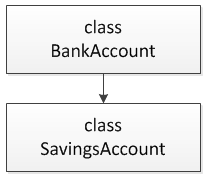
\includegraphics[scale=0.5]{img/single_inheritance.png}   \\
\vspace{2em}
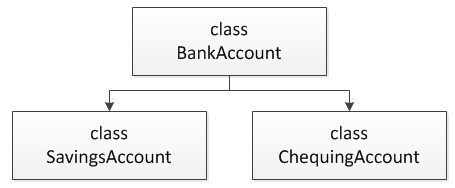
\includegraphics[scale=0.5]{img/single_inheritance_2.png}   \\

&&

\raggedright
\begin{footnotesize}
Java uses \textbf{single inheritance}, which means a subclass can extend a single superclass. \\
\vspace{1em}
In single inheritance, any number of subclasses can have the same superclass. \\
\end{footnotesize}

\end{splitslide}
\end{frame}
%%%%%%%%%%%%%%%%%%%%%%%%%%%%%%%%%%%%%%%%%%%%%%%%%%%%%%%%%%%%%%%%%%%%%%%%%%%%%%%%%%%



%%%%%%%%%%%%%%%%%%%%%%%%%%%%%%%%%%%%%%%%%%%%%%%%%%%%%%%%%%%%%%%%%%%%%%%%%%%%%%%%%%%
% Inheritance (more info)
%%%%%%%%%%%%%%%%%%%%%%%%%%%%%%%%%%%%%%%%%%%%%%%%%%%%%%%%%%%%%%%%%%%%%%%%%%%%%%%%%%%
\begin{frame}[fragile]{Inheritance}
\begin{splitslide}

\centering
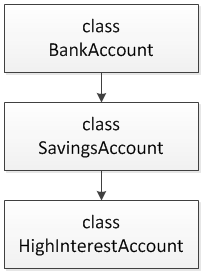
\includegraphics[scale=0.5]{img/multilevel_inheritance.png}   \\

&&

\raggedright
\begin{footnotesize}
Java also has \textbf{multi-level inheritance}, which means subclasses can themselves be subclassed. \\
\end{footnotesize}

\end{splitslide}
\end{frame}
%%%%%%%%%%%%%%%%%%%%%%%%%%%%%%%%%%%%%%%%%%%%%%%%%%%%%%%%%%%%%%%%%%%%%%%%%%%%%%%%%%%



%%%%%%%%%%%%%%%%%%%%%%%%%%%%%%%%%%%%%%%%%%%%%%%%%%%%%%%%%%%%%%%%%%%%%%%%%%%%%%%%%%%
% Inheritance (more info)
%%%%%%%%%%%%%%%%%%%%%%%%%%%%%%%%%%%%%%%%%%%%%%%%%%%%%%%%%%%%%%%%%%%%%%%%%%%%%%%%%%%
\begin{frame}[fragile]{Inheritance}
\begin{splitslide}

\centering
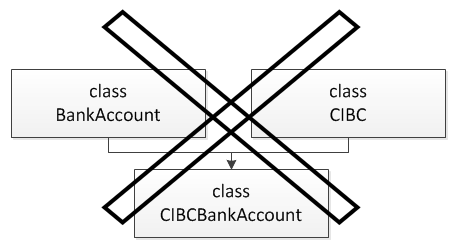
\includegraphics[scale=0.5]{img/multiple_inheritance.png}   \\

&&

\raggedright
\begin{footnotesize}
Java does \textbf{not} allow \textbf{multiple inheritance}...a class cannot inherit from multiple classes. \\
\vspace{0.5em}
There are certainly times where we want classes to take on behaviours or characteristics from multiple sources...there are better ways to do this that we will see. \\
\end{footnotesize}

\end{splitslide}
\end{frame}
%%%%%%%%%%%%%%%%%%%%%%%%%%%%%%%%%%%%%%%%%%%%%%%%%%%%%%%%%%%%%%%%%%%%%%%%%%%%%%%%%%%



%%%%%%%%%%%%%%%%%%%%%%%%%%%%%%%%%%%%%%%%%%%%%%%%%%%%%%%%%%%%%%%%%%%%%%%%%%%%%%%%%%%
% Polymorphism (definition)
%%%%%%%%%%%%%%%%%%%%%%%%%%%%%%%%%%%%%%%%%%%%%%%%%%%%%%%%%%%%%%%%%%%%%%%%%%%%%%%%%%%
\begin{frame}{Characteristics of OOP}
	\begin{description}
		\item[Polymorphism]
		A subclass can override (replace) a method inherited from the superclass with its own version.
	\end{description}
\end{frame}
%%%%%%%%%%%%%%%%%%%%%%%%%%%%%%%%%%%%%%%%%%%%%%%%%%%%%%%%%%%%%%%%%%%%%%%%%%%%%%%%%%%

%%%%%%%%%%%%%%%%%%%%%%%%%%%%%%%%%%%%%%%%%%%%%%%%%%%%%%%%%%%%%%%%%%%%%%%%%%%%%%%%%%%%
% Polymorphism (overriding)
%%%%%%%%%%%%%%%%%%%%%%%%%%%%%%%%%%%%%%%%%%%%%%%%%%%%%%%%%%%%%%%%%%%%%%%%%%%%%%%%%%%%
\begin{frame}[fragile]{Polymorphism}
\begin{splitslide}

\begin{Verbatim}[fontsize=\tiny]
public class BankAccount {
  protected double balance;
  
  // constructor
  public BankAccount(double opening_balance) {
    balance = opening_balance;
  }
  
  // deposit an amount
  public void deposit(double amount) {
    balance += amount;
  }
  
  // withdraw an amount
  public boolean withdraw(double amount) {
    if(balance < amount) {
      return false;
    }
    else {
      balance -= amount;
      return true;
    }
  }
}
\end{Verbatim}

&&

\begin{Verbatim}[fontsize=\tiny]
class SavingsAccount extends BankAccount {
  private double interest_rate = 0.008;
  
  // apply the interest rate
  public void apply_interest() {
    balance *= interest_rate;
  }
}

class HighInterestAcct extends BankAccount {
  private double withdrawl_fee = 1.50;
  
  // override withdraw to add a fee
  public boolean withdraw(double amount) {
    int debit = amount + withdrawl_fee;    
    if(balance < debit) {
      return false;
    }
    else {
      balance -= debit;
      return true;
    }
  }
}
\end{Verbatim}

\end{splitslide}
\end{frame}
%%%%%%%%%%%%%%%%%%%%%%%%%%%%%%%%%%%%%%%%%%%%%%%%%%%%%%%%%%%%%%%%%%%%%%%%%%%%%%%%%%%%

%%%%%%%%%%%%%%%%%%%%%%%%%%%%%%%%%%%%%%%%%%%%%%%%%%%%%%%%%%%%%%%%%%%%%%%%%%%%%%%%%%%%
% Objects
%%%%%%%%%%%%%%%%%%%%%%%%%%%%%%%%%%%%%%%%%%%%%%%%%%%%%%%%%%%%%%%%%%%%%%%%%%%%%%%%%%%%
\begin{frame}[fragile]{Objects}
Classes aren't any good unless we can use them. \\
An object is an \textbf{instance} of a class.   \\
Like variables, we can make as many instances of as many classes as memory allows. \\
	
\end{frame}
%%%%%%%%%%%%%%%%%%%%%%%%%%%%%%%%%%%%%%%%%%%%%%%%%%%%%%%%%%%%%%%%%%%%%%%%%%%%%%%%%%%%

\section{Working with Java Classes}

%%%%%%%%%%%%%%%%%%%%%%%%%%%%%%%%%%%%%%%%%%%%%%%%%%%%%%%%%%%%%%%%%%%%%%%%%%%%%%%%%%%%
% Creating Objects
%%%%%%%%%%%%%%%%%%%%%%%%%%%%%%%%%%%%%%%%%%%%%%%%%%%%%%%%%%%%%%%%%%%%%%%%%%%%%%%%%%%%
\begin{frame}{Creating objects}
\begin{itemize}
\item A \textbf{constructor} is a method that each class invokes when an instance is created
\item Constructors can be overloaded (we can have more than one for a given class)
\end{itemize}
\end{frame}

\end{document}